\section{Evaluation and Results}\label{sec:evaluation}
%
% ~\textcolor{red}{q. this para can be removed for shortening perhaps}In our experiments we study (i) whether our method can infer 
% programs to translate instructions to desired goal states, 
% (ii) the extent to which the method generalizes to novel 
% instructions and world states and (iii) whether the model 
% can generalize to multiple step plans having been trained on 
% simpler plans and (iv) whether model predictions can be used by a simulated 
% robot to execute a task as well as hypothesize future world states. 

% Main accuracy results
\begin{table*}[ht]
    \centering
    \caption{Comparison between Proposed Model and NMN+  (BB: Bounding Boxes)}
    \begin{tabular}{|c|c|c|c|c|c|c|c|c|c|c|c|c|}
    \hline
         Model  & \multicolumn{3}{|c|}{Overall} &  \multicolumn{2}{|c|}{Single-step} & \multicolumn{2}{|c|}{Double step} & \multicolumn{2}{|c|}{Simple} & \multicolumn{2}{|c|}{Complex} \\ 
         \hline
         \hline
          & IOU & IOU-M & Program & IOU & IOU-M  & IOU & IOU-M  & IOU & IOU-M & IOU & IOU-M  \\
           &  &  & (Action/Subj/Pred) & &   &  & &  &  &  &   \\
          \hline
         NMN+ (gold BB) & 0.77 & 0.55 & --/0.81/0.76 & 0.80 & 0.56 &    0.71 & 0.52 &0.90 & 0.71 & 0.64 & 0.31\\ 
         \hline 
         Ours (gold BB)  & 0.87 & 0.72& 0.99/0.99/0.94 & 0.91 & 0.64 &   0.87 & 0.62 & 0.92 & 0.73 & 0.87 & 0.64 \\
        \hline 
         NMN+ (extracted BB) & 0.69 & 0.32& --/0.81/0.55 & 0.78 & 0.49 &  0.58 & 0.22 & 0.79 & 0.55 & 0.60 & 0.20\\ 
         \hline 
         Ours (extracted BB) & 0.76  & 0.41  & 0.99/0.74/0.76 &0.80 & 0.43  & 0.69 & 0.54  & 0.83 & 0.62 & 0.69 & 0.24\\
         \hline 
    \end{tabular}
    % \vspace{1em}
    \label{tab:accuracy}
\end{table*} 

%%%%%%%%%%%%%%%%%%%%%%%%%%%
%%% EXPERIMENTAL SETUP %%%
%%%%%%%%%%%%%%%%%%%%%%%%%%%

% \begin{table*}[ht]
%     \centering
%     \caption{Accuracy Comparison for the Proposed Model and the Baseline}
%     \begin{tabular}{|c|c|c|c|c|c|c|c|c|c|c|c|c|c|c|c|c|}
%     \hline
%          Model  & \multicolumn{3}{|c|}{Overall} &  \multicolumn{3}{|c|}{Single-step} & \multicolumn{3}{|c|}{Double step} & \multicolumn{3}{|c|}{Simple} & \multicolumn{3}{|c|}{Complex} \\ 
%          \hline
%          \hline
%           & IOU & IOU-M & & Program & IOU & IOU-M & Program &  IOU & IOU-M & Program & IOU & IOU-M & Program & IOU & IOU-M  & Program \\
%           \hline
%          Baseline & 0.77 & 0.55 & 0.80 & 0.56 & 0.71 & 0.52 & 0.90 & 0.71 & 0.64 & 0.31\\ 
%          \hline 
%          Ours  & 0.87 & 0.72 & 0.91 & 0.64 & 0.87 & 0.62 & 0.92 & 0.73 & 0.87 & 0.64 \\
%         \hline 
%          Baseline + Perception & 0.69 & 0.32 & 0.78 & 0.49 & 0.58 & 0.22 & 0.79 & 0.55 & 0.60 & 0.20\\ 
%          \hline 
%          Ours + Perception & 0.76  & 0.41  & 0.80 & 0.43 & 0.69 & 0.54 & 0.83 & 0.62 & 0.69 & 0.24\\
%          \hline 
%     \end{tabular}
%     % \vspace{1em}
%     \label{tab:accuracy}
% \end{table*} 



% \begin{table}
%     \centering
%     \caption{Comparison of Proposed Model and CLIPort}
%     \begin{tabular}{|c|c|c|}
%          \hline 
%          Model  & Identification Accuracy & Placement Accuracy \\ 
%          \hline
%           CLIPort & 0.46 &  0.39  \\
%           \hline
%          CLIPort(x5) &  & \\ 
%          \hline 
%          Ours    & 0.94 & 0.93 \\
%         \hline 
%     \end{tabular}
%     % \vspace{1em}
%     \label{tab:cliport}
% \end{table} 


\begin{table}[ht]
    \large
    \centering
    \caption{Comparison b/w Proposed Model and CLIPort}
    \resizebox{\columnwidth}{!}{%   
    \begin{tabular}{|c|c|c|c|c|c|c|c|c|c|c|c|c|}
    \hline
         Model  & \multicolumn{2}{|c|}{Overall}  & \multicolumn{2}{|c|}{Simple} & \multicolumn{2}{|c|}{Complex} \\ 
         \hline
         \hline
          & Id. Acc. & Pl. Acc. & Id. Acc.  & Pl. Acc. & Id. Acc.  & Pl. Acc.   \\
          
          \hline
            CLIPort & 0.46 & 0.39 & 0.55 & 0.47 & 0.32 &    0.26 \\ 
         \hline 
                     CLIPort(5x) & 0.76 & 0.61 & 0.90 & 0.74 & 0.55 &    0.39 \\ 
                     \hline 
         Ours (gold BB)  & 0.94 & 0.93 & 1.0 & 1.0  & 0.83 & 0.81  \\
         \hline 
    \end{tabular}%
    }
    % \vspace{-0.25in}
    \label{tab:cliport}
\end{table} 





\subsection{Experimental Setup}
%%% DATA %%%
\textbf{Data collection. } 
The dataset is collected in a PyBullet tabletop environment using a 
simulated Franka Emika Panda robot arm. The workspace consists of a tabletop with blocks of different shapes and colors.
%
Each datapoint consists of an initial scene paired with a language instruction and the expected resulting final scene. 
For training, close to 5000 synthetic scenes and language instructions(with a 80:20 train-test split) are sampled with 3-5 blocks of varying colors and shapes and placed at randomized orientations on the table. 
%
% The instructions range from single physical pick-place operation \emph{``Put the red block on the green block"} to ones involving a composition of such operations like \emph{``Put the red block which is behind the white dice to right of the blue cube, then put the lego block on top of red block"}. 
%
%The robot's motion skills are realized using a crane grasping for
%picking and re-positioning the object at the target pose.

The dataset consists of both single-step(e.g. \emph{``Put the red block on the green block"}) and double step commands(e.g. \emph{``Put the red block which is behind the white dice to right of the blue cube, then put the lego block on top of red block"}). 
On the basis of the level of reasoning involved in the given instruction, we can classify the dataset into (i) \textit{simple} that involve reasoning over individual object features only and \textit{complex} that additionally involve reasoning over inter-object relationships.

%%% BASELINE %%%
\subsection{Baselines, Metrics and Comparisons} 
The proposed model (i) performs visuo-linguistic reasoning in a symbolic latent space and (ii) assumes an object-centric state representation. We provide comparisons with baselines that forego these two assumptions.

% \textbf{CLIPort}~\cite{shridhar2022cliport} performs language-guided manipulation by leveraging the visual and linguistic semantics embedded in pre-trained CLIP~\cite{clip}. Unlike ours, the model lacks explicit, modular constructs to perform the reasoning inherent in object manipulation tasks.} ~\textcolor{red}{TODO: Add explanation for table3 

\textbf{NMN+}, inspired from Neural Module Networks \cite{andreas2016neural}, assumes an object-centric state representation. However, in contrast to the proposed model, visuo-linguistic reasoning required for manipulation is performed using language-guided attention over object embeddings instead of using symbolic reasoning constructs. Figure~\ref{fig:nmn} provides the detailed architecture. The entire architecture is neural and is trained end-to-end with the loss same as that of the proposed model. 

% For a fair evaluation, our model and the baseline share the instruction encoder, the action simulator and the object feature extractor. The baseline includes an action decoder and four attention modules divided into two groups of two each. Each group takes in the encoded instruction and embedding for all objects present in scene and predicts two objects involved in manipulation. The location of the predicted objects and output of the action decoder is the input to the action decoder, that provides the predicted location as output. Here, \textit{location} includes both the bounding box and depth of the object. 



\begin{figure}
\begin{subfigure}{1.0\hsize}
     \centering    
     \includegraphics[scale=0.19]{figures/baseline.png}
\end{subfigure}
\caption{
    \footnotesize{
        \textbf{Object-centric baseline NMN+.} For a fair comparison, our model and NMN+ share the same language encoder (with LSTM-based splitter) and the visual extractor. Attention blocks compute language-guided attention over object embeddings to get the \emph{subject} and \emph{predicate} for the manipulation action. This is fed into the action simulator along with the action embedding from the action decoder to get the predicted final location of the object.}}
        \vspace{-0.15in}
            \label{fig:nmn}
\end{figure}

The following metrics are used for comparing the proposed model with \emph{NMN+}:
(i) \emph{Intersection over Union (IOU)} of the predicted and groundtruth bounding box is calculated in the 2D image space assuming a static camera viewing the scene. Average IOU over all objects in the scene and mean IOU for objects moved during execution, termed IOU-M,  are reported.  
(ii) \emph{Program Accuracy}: The grounded program inferred for an (instruction, scene)-pair using the proposed model is compared with the manually annotated ground truth program. We separately report the grounding accuracy for the subject and predicate of our action (assumed binary) and the accuracy of the predicted action inferred from the instruction. Since, there is no explicit notion of grounded actions in the baseline, we do not report this metric for the baseline. 

\begin{figure}[h!]
\begin{subfigure}{0.5\hsize}
     \centering    
     \includegraphics[scale=0.19]{figures/multi-object-1.png}
    \caption{\footnotesize{IoU vs \# of objects}}
    % IoU of the predicted position of the object moved during execution with its ground truth position v/s number of objects in the scene.
    \label{fig:large_scenes}
\end{subfigure}%
% Generalization on larger steps
% \begin{figure}[!h]
%     \centering
%     \subfigure{\includegraphics[width=0.2\textwidth]{figures/large_steps.png}} 
%     \subfigure{\includegraphics[width=0.2\textwidth]{figures/generalization_large_scenes.png}} 
%     \caption{Caption}
%     % \label{fig:foobar}
% \end{figure}
\begin{subfigure}{0.5\hsize}
     \centering    
     %\includegraphics[height=4.375cm,width=3cm]{figures/multi-step.png}
    \includegraphics[scale=0.19]{figures/multi-step-1.png}
    \caption{\footnotesize{IoU vs varying \# of steps}}
     %IoU of the predicted position of the object moved during execution with its ground truth position v/s number of atomic actions implied in the instruction.
    \label{fig:large_steps}
\end{subfigure}
\caption{\footnotesize{Performance in generalization settings}}
\vspace{-0.15 in}
\end{figure}


\begin{figure*}[hbt!]
    \centering    
    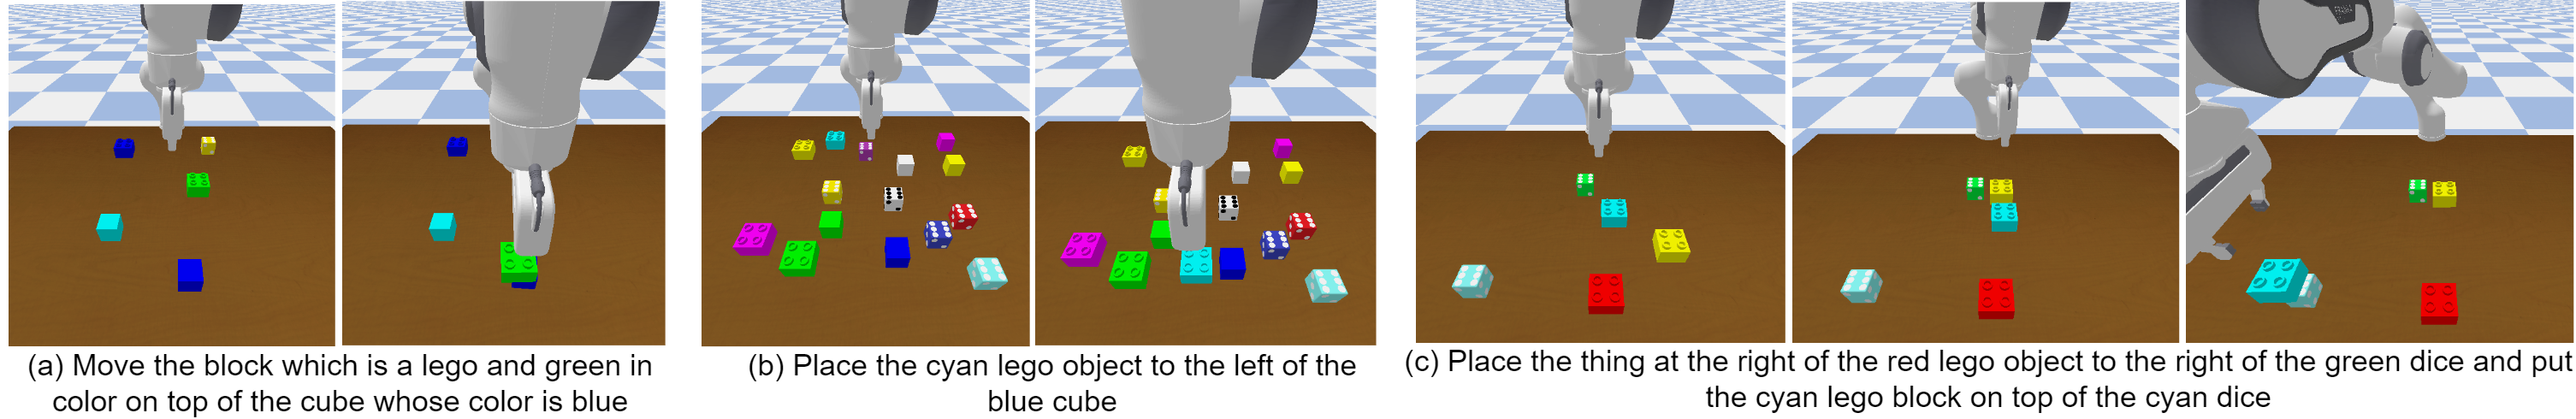
\includegraphics[width=16.5cm]{figures/row2a.png}
    % \caption{
    % \footnotesize{
    % }}
    \label{fig:qual-1}
\end{figure*}
\begin{figure*}[hbt!]
    \centering    
    \includegraphics[width=17cm]{figures/row2b.png}
    \caption{
    \footnotesize{
    Execution of robot manipulator on (a) compound instructions, (b) scene with 15 objects, (c) double step instruction with relational attributes, (d) 5-step instruction. (d) also shows reconstruction of the predicted scene before each step of the simulation
    }}
    \label{fig:qual-1}
    \vspace{-0.1 in}
\end{figure*}


Table \ref{tab:accuracy} reports the performance of our model and the baseline on the test set. We report both numbers: using gold set of bounding boxes and using bounding boxes extracted~\footnote{Excluded about 10\% no detection cases for both models.} using the approach described in Section~\ref{subsec:visual-reason}. Our model outperforms the baseline overall. For instructions with complex reasoning (resolution of binary spatial relations) involved, the proposed model outperforms the baseline by $33$ points in the IOU-M metric.
%
Disentangled representations of relations and concepts in \textit{Visual Reasoning} module allow the proposed model to reason over complex instructions.

\textbf{CLIPort}~\cite{shridhar2022cliport} takes as input a dense, image-based state representation, in contrast to our object-centric state representation. It proposes a two-stream architecture that computes language-guided attention masks on the input scene for both pick and place locations. It lacks explicit symbolic constructs for reasoning about the scene. Instead, the reasoning required for manipulation is performed by leveraging the visuo-linguistic understanding of the large pre-trained model CLIP ~\cite{clip}. Table ~\ref{tab:cliport} compares \emph{CLIPort} with our model. Since \emph{CLIPort} performs only single-step pick-and-place operations, the numbers are calculated only on single-step examples. The following metrics are used (i) \emph{Placement Accuracy}: fraction of examples in which the predicted place location lies within the groundtruth bounding box of the moved object (ii) \emph{Identification Accuracy}: fraction of examples in which the predicted pick location lies within the groundtruth bounding box of the moved object. For the proposed model, the centre of the predicted bounding box location is used as the predicted place location.

We observe that CLIPort on our dataset shows low accuracy in both predicting the object to be moved as well as the place location. Further, its performance deteriorates in examples with relational concepts. We note that the performance and sample-efficiency of CLIPort critically depends upon  spatial consistency of input images i.e. objects do not scale or distort depending on the viewing angle as in ~\cite{shridhar2022cliport}. To provide additional leverage to the baseline, we train CLIPort on 5 times more data than the original, results of which are reported under the title CLIPort-5x. We observe an improvement in performance on the larger dataset, although still worse than that of the proposed model. 
% This can be attributed to (i) its inability to learn from sparse dataset (due to lack of modularity), (ii) the use of raw image as state representation, and (iii) lack of spatial consistency in images, i.e. objects can scale or distort depending on the viewing angle,  in contrast to the setting used by CLIPort. To further establish CLIPort's data inefficiency, we train it with 5 times more data. Specifically, for each scene in the original dataset, we add 5 additional instructions and corresponding final scenes. This leads to improvement in performance, although inferior to that of the proposed model. 


%
%% Generalization on Larger Scenes

%% Main Results
%%%%%%%%%%%%%%%
% \subsection{Model Accuracy}
% % Quantitative evaluation
% %\textbf{Quantitative Evaluation.} 
% A quantitative evaluation of model accuracy is is carried out in two settings. First, we use a $80:20$ train:test split of the entire corpus for accuracy comparison. The corpus consists of both single step and double step commands, along with sentences of different complexities:- \textit{simple} and \textit{complex}. Complex sentences involve reasoning on inter-object relationships, while simple sentences reason over individual object features only. 




% We demonstrate our model's ability to infer a sequence of grounded sub-goals, given an initial scene and instruction, that involves manipulating the scene over multiple time step and complex multi-hop reasoning.
% %
% Table \ref{tab:accuracy} reports the performance of our model and the baseline on the test set. We report both numbers: using gold set of bounding boxes and using bounding boxes extracted~\footnote{Excluded about 10\% no detection cases for both models.} using the approach described in Section~\ref{subsec:visual-reason}. Our model outperforms the baseline overall. For instructions with complex reasoning (resolution of binary spatial relations) involved, the proposed model outperforms the baseline by $33$ points in the IOU-M metric.
% %
% Disentangled representations of relations and concepts in \textit{Visual Reasoning} module allow the proposed model to reason over complex instructions. 

% For the remaining experiments, the numbers are reported using gold BBs for both the models.


% \texttt{Single-step} and \texttt{Double Step} refer to instructions with one and two actions involved resprectively and \texttt{Simple reasoning} refers to simple reasoning bases upon 
% reports the accuracy results. Both test (around 1700 samples) and train set (around 1700 samples) contain 1 - 2 step commands. Further, test and train do not have any 1-step command in common. Both models achieve a high accuracy during training but the proposed model shows significant improvement over the baseline for the test set.  
%
% Overall Accuracy on Test and Train Sets
%\subsection{Generalization With Increasing Scene Objects}
% The proposed model is able to interpret the correct object and move it to the correct position with marginal decline in performance to scenes with up to 10 objects after being trained on scenes with up to 5 objects only, without any obtrusive decrease in accuracy. Disentangled representations of object features and spatial features in the scene graph extracted by the \textit{Visual Reasoner} from the scene along with an object-centric view of the environment help the model to generalise strongly to larger number of objects. 


%%%%% Generalization
\subsection{Combinatorial Generalization} 

To evaluate the approaches in an out-of-distribution generalization setting, we collect dataset consisting of scenes with more objects than seen during training, and with instructions that involve larger number of steps for carrying out the task.

Figure~\ref{fig:large_scenes} illustrates the model generalizing combinatorially to scenes with more number of objects. The models were first trained on scenes having up to $5$ objects only, and then tested on scenes having up to $10$ objects.\\ 
%
The superior generalization demonstrated by the model can be attributed to reliance on an object-centric state representation and the ability to learn dense disentangled representations of spatial and action concepts, facilitating modular and structured reasoning that scales gracefully. 

Figure ~\ref{fig:large_steps} illustrates model generalization to longer horizon manipulation. We observe that the proposed model is able to perform multiple scene manipulation and reasoning steps with considerable accuracy up to $7$ steps after being trained with instructions translating to plans up to $2$ steps.\\ 
%
The performance of the object-centric baseline (NMN+) is worse and the model struggles to generalize to plans extending to longer horizons. We attribute this to the modular structure of our approach compared to the baseline.
\iffalse
\begin{figure}[h]
    \centering    
    \includegraphics[width=7.5cm]{figures/rel.png}
    \caption{
    \footnotesize{Execution of robot manipulator on a double step instruction containing relational attributes: \emph{Place the thing at the right of the red lego object to the right of the green dice and put the cyan lego block on top of the cyan dice}
    }}
    \label{fig:relative}
\end{figure}
\fi
%
\subsection{Demonstration on a Simulated Robot}
%
We demonstrate the learned model for interpreting instructions 
provided to a simulated 7-DOF Franka Emika manipulator in a table top setting. 
%
The robot is provided language instructions and uses the model to predict a program that once executed transitions the world state to the intended one. The 2-D bounding boxes predicted by the action simulator are translated to 3-D coordinates in the world space via a learned MLP using simulated data.
%
The predicted positions are provided to a low-level motion planner for trajectory generation with crane grasping for picking/placing. 
%Each step of the robot simulation is then performed by grasping the object at the initial location, moving the gripper to the final predicted location, and releasing the gripped object. 
% 
Figure \ref{fig:qual-1} shows execution by the robot manipulator on complex instructions, scenes having multiple objects, double step relational instructions, and multi-step instructions. We also visualise reconstruction of the moved objects before each step of the actual execution. The structural similarity index (SSIM) \cite{ssim2004} for the reconstruction model is 0.935.
% omitted since we do not have space
%Figure \ref{fig:relative} demonstrates model performance on an instruction containing relational attributes.
%



\iffalse
\subsection{Failure cases}
In roughly 10\% of examples in the dataset, the object detector returns a false object proposal, or misses an object, in either of initial or final scenes. Since we are unable to calculate loss in such cases, these examples are not considered for experiments with perception.
\fi

%%%% ATTIC %%%%
\iffalse

% Table~\ref{tab:accuracy} reports the performance of our model and the baseline on the test set. 
% reports the accuracies for the proposed and the 
% baseline models. The results indicate a stronger generalization for the proposed approach compared to the baseline model.
%
% The result illustrates the model’s ability to reason about language instructions with novel object attribute references in the context of the scene. Such visual-linguistic reasoning operates on a single scene. Next, we assess generalization over multiple time steps. We explicitly evaluate the model on a test cases where an instruction involves multi-step actions that exceed those seen in training.

% %  \vspace{-2em}
% \begin{table}
%     \centering
%     \caption{Generalization On Instructions with Novel Object Attributes}
%     \begin{tabular}{|c|c|c|c|c|c|c|c|}
%     \hline
%     Model & Prog ($P$) & Arg ($O_1$) & Arg ($O_2$) & IOU-2D & IOU-3D \\ \hline \hline
%     Baseline & - & 87.5 & 89.1 & 29.0 & 16.6 \\ 
%     Ours &  98.5 & 96.3 & 96.3 & 51.6  & 25.2  \\
%    \hline
%     \end{tabular}
%     \label{tab:generalization-attributes}
% \end{table}
% %
%  \vspace{-0.5em}
% \begin{table}
%     \centering
%     \caption{Generalization over Three-step Instructions with One/Two-step Instructions in Training}
%     \begin{tabular}{|c|c|c|c|c|c|}
%     \hline
%     %Model &$P$ & ($P_g$) & ($o_1$) & ($o_2$) & IOU-2D & IOU-3D \\ 
%     Model & Prog ($P$) & Arg ($O_1$) & Arg ($O_2$) & IOU-2D & IOU-3D \\
%     \hline \hline
%     Baseline & - & 76.0  & 80.9 & 13.3 &  6.6  \\
%     Our & 56.8  & 54.7 & 53.6 & 27.2 & 12.9 \\
%     % Random & 12.5 & 0.09 & 3.4 & 3.4 & - & -\\
%     \hline
%     \end{tabular}
%     \label{tab:generalization-multi-step}
% \end{table}

% Table~\ref{tab:generalization-multi-step} presents the results. The models were only trained on 1-2 step commands, and are tested on 3 step commands. The proposed model shows improved generalization compared to the baseline in the IOU metrics. 

% %  \vspace{-2em}
% \begin{table}
%     \centering
%     \caption{Generalization to Novel Multi-Object Attribute Instructions}
%     \begin{tabular}{|c|c|c|c|c|c|}
%     \hline
%         Model & Prog ($P$) & Arg ($O_1$) & Arg ($O_2$) & IOU-2D & IOU-3D \\\hline \hline
%         %Model & ($P$) & ($o_1$) & ($o_2$) & IOU-2D & IOU-3D \\  \hline \hline
%         Baseline & - &55.0 &32.4 & 3.2& 1.5\\
%       Ours & 98.0 & 75.7 & 89.5 & 27.3 & 9.3 \\ \hline 
%     %   Baseline & 84.3 & 90.2 & 93.0 & 49.0 & 30.3     \\\hline
%     \end{tabular}
%     % \vspace{1em}
    \label{tab:generalization-multiple-object-attributes}
% \end{table}

% Table~\ref{tab:generalization-multiple-object-attributes} presents evaluation on task instructions that involve multi-step reasoning over attributes in the setting where the model is trained 
% only on a single attribute. For example, the training set instructions only involve singe 
% attributes such as 'red' and 'lego' with two different objects but during testing the model must compositional reason over both attributes to understand and follow the instruction. As before, 
% the ability to combine grounded concepts with reasoning allows the proposed model to generalize 
% better in this setting achieving significantly higher generalization accuracy compared to the baseline. 

% The above results demonstrate stronger generalization to novel scenes with unseen object attribute pairs as well as action sequences that extend beyond those encountered during training. 
% %
% The neuro-symbolic approach involves learning of data-driven learning of concept representations that are amenable to rich compositional reasoning. The neuro-symbolic approach transfers better to novel settings compared to the direct neural-only approach that does not make use of the modular structure during training.

\begin{figure}[ht]
    \centering
    \setlength\tabcolsep{1.5pt}
    \begin{tabular}{ccc}
      \includegraphics[width=28mm]{figures/1step/rgba0002.png} &   \includegraphics[width=28mm]{figures/1step/rgba0009.png} &
      \includegraphics[width=28mm]{figures/1step/rgba0017.png}\\
    % \multicolumn{2}{c}{\includegraphics[width=55mm]{it} }\\
    % \multicolumn{2}{c}{(e) fifth}
    \end{tabular}
    \caption{A robot manipulator correctly performing a single step instruction \emph{``put cyan block on blue block"} in a simulated table top environment. }
    \label{fig:demo-1}
\end{figure}

%
Figure~\ref{fig:demo-1} illustrates the robot successfully performing a single step instruction, \emph{``put cyan block on the blue block"} using the sub-goal predicted by the inferred program. 

%
Figure~\ref{fig:demo-2} illustrates the robot manipulator performing the instruction \emph{``put yellow block to the left of white block and put magenta small block on yellow block"}. the model reasons about the input instruction in the context of the environment correctly positions the yellow block on the left side of the intended white block. Subsequently, the robot grasps the magenta block and correctly positions the block on the yellow block that was previously manipulated. 

\begin{figure}
    \centering
    \setlength\tabcolsep{1.5pt}
    \begin{tabular}{ccc}
       \includegraphics[trim={5cm 5cm 5cm 0},clip,width=28mm]{figures/2step_s/rgba0002.png}  &
       \includegraphics[trim={5cm 5cm 5cm 0},clip,width=28mm]{figures/2step_s/rgba0006.png}  &
       \includegraphics[trim={5cm 5cm 5cm 0},clip,width=28mm]{figures/2step_s/rgba0011.png} \\
       \includegraphics[trim={5cm 5cm 5cm 0},clip,width=28mm]{figures/2step_s/rgba0015.png} &
       \includegraphics[trim={5cm 5cm 5cm 0},clip,width=28mm]{figures/2step_s/rgba0020.png} &
       \includegraphics[trim={5cm 5cm 5cm 0},clip,width=28mm]{figures/2step_s/rgba0021.png} 
    \end{tabular}
    \caption{Robot manipulator performing a two-step instruction \emph{``put yellow block to the left of white block and put magenta small block on yellow block"}}
    \label{fig:demo-2}
\end{figure}
%Further, note that the model used in the demonstrates shown in 
%Figures~\ref{fig:demo-2} and~\ref{fig:demo-2} 

% Incorrect: multi step instruction. 
\begin{figure}
    \centering
    \setlength\tabcolsep{1.5pt}
    \begin{tabular}{ccc}
       \includegraphics[trim={5cm 5cm 5cm 0},clip,width=28mm]{figures/2step_f/rgba0002.png}  &  
       \includegraphics[trim={5cm 5cm 5cm 0},clip,width=28mm]{figures/2step_f/rgba0008.png}  &
       \includegraphics[trim={5cm 5cm 5cm 0},clip,width=28mm]{figures/2step_f/rgba0016.png} \\
       \includegraphics[trim={5cm 5cm 5cm 0},clip,width=28mm]{figures/2step_f/rgba0026.png} &
       \includegraphics[trim={5cm 5cm 5cm 0},clip,width=28mm]{figures/2step_f/rgba0031.png} &
       \includegraphics[trim={5cm 5cm 5cm 0},clip,width=28mm]{figures/2step_f/rgba0034.png} \\
    %   \multicolumn{3}{c}{Robot manipulator performing a double step instruction \emph{"put red block on blue block and put magenta block on red block"}. The robot correctly inferred the sequence of symbolic actions but failed during execution error due to the unstable placement of the second block. }
    \end{tabular}
    \caption{Robot manipulator performing a two-step instruction \emph{"put red block on blue block and put magenta block on red block"}. The robot correctly inferred the sequence of symbolic actions but failed during execution error due to the unstable placement of the second block. }
    \label{fig:demo-3}
\end{figure}

%
Figure~\ref{fig:demo-3} shows the execution for the instruction \emph{``put red block on blue block and put magenta block on red block"}. The model correctly predicts a program consisting of a composition of two sequential manipulation actions. The robot correctly identifies the intended objects for manipulation, then grasps and re-positions them to form the intended assembly. In the final step, the robot correctly placed the magenta-colored block on top of the red-colored block, however, the inferred placement was unstable and the block fell from the assembly. Note that the current model infers the task plan which is then handed over to the motion planner. Such a staged approach possesses the inherent limitation of not being able to recover from execution failures. The possibilities of a reactive approach by interleaving planning and execution are to be explored in future work and is likely to benefit error-recovery.

%
In Figure~\ref{fig:demo-4}, the robot is provided with the instruction, \emph{``put red block to the left of yellow block and put cyan block to the left of red block and then put red block on cyan block"} which requires three successive manipulations. The model used in this experiment is trained only on two step instructions. However, at inference time, the model can generalize to a longer instruction by leveraging the compositionality inherent in our program representation. 


\begin{figure}
    \centering
    \setlength\tabcolsep{1.5pt}
    \begin{tabular}{ccc}
       \includegraphics[trim={5cm 5cm 5cm 0},clip,width=28mm]{figures/3step_s/rgba0002.png} &  
       \includegraphics[trim={5cm 5cm 5cm 0},clip,width=28mm]{figures/3step_s/rgba0011.png}  &
       \includegraphics[trim={5cm 5cm 5cm 0},clip,width=28mm]{figures/3step_s/rgba0015.png} \\
       \includegraphics[trim={5cm 5cm 5cm 0},clip,width=28mm]{figures/3step_s/rgba0020.png} &
       \includegraphics[trim={5cm 5cm 5cm 0},clip,width=28mm]{figures/3step_s/rgba0025.png} &
       \includegraphics[trim={5cm 5cm 5cm 0},clip,width=28mm]{figures/3step_s/rgba0030.png} \\
    \end{tabular}
    \caption{Robot manipulator performing a three-step instruction \emph{``put red block to the left of yellow block and put cyan block to the left of red block and then put red block on cyan block"}. The robot correctly inferred the sequence of actions. }
    \label{fig:demo-4}
\end{figure}
\fi


% \begin{figure*}[hbt!]
%     \centering    
%     \includegraphics[width=15cm]{figures/qualitative.png}
%     \caption{
%     \footnotesize{Execution of robot manipulator on a 5-step instruction: \emph{Put the blue lego thing on the left side of the red lego thing and place the red cube on the left side of the white lego object and move the magenta dice to the right of the green box and move the red box on the left side of the blue lego thing and put the blue lego object to the left of the white lego thing}. The first row shows the scene after each action in the robot simulation. The second row shows reconstruction of the predicted scene before each step of the simulation
%     }}
%     \label{fig:qualitative}
% \end{figure*}
